\documentclass[12pt,a4paper]{article}

\usepackage[utf8]{inputenc}
\usepackage[T1]{fontenc}
\usepackage[spanish]{babel}
\usepackage{amsmath}
\usepackage{graphicx}
\usepackage[margin=2.5cm]{geometry}
\title{Caracterizaci\'on del pico de $^{40}$K en Mg4 con HPGe \\
(calibraci\'on multipunto con 5 l\'ineas de fondo)}
\author{Laboratorio Nuclear}
\date{\today}

\begin{document}
\maketitle

\section*{Objetivo}
Identificar y caracterizar el fotopico de $^{40}$K en el espectro HPGe de la
muestra Mg4, usando el ajuste gaussiano implementado en
\texttt{src/gaussian\_background.f}.
La calibraci\'on en energ\'{\i}a se obtiene por regresi\'on lineal de 5 anclas
identificadas visualmente en el espectro: $^{7}$Be/$^{228}$Ac/$^{238}$U
(114.673~keV), $^{226}$Ra (186.211~keV), $^{212}$Pb (238.632~keV),
$^{40}$K (1460.820~keV) y $^{208}$Tl (2614.511~keV).
Se verifica la concordancia de las 14 l\'{\i}neas del fondo
(\texttt{fondo\_GeHP\_BEGe.dat}) con esta calibraci\'on,
reportando las discrepancias observadas.

\section*{Datos y m\'etodo}
Se analiz\'o el archivo \texttt{Mg4/datos/Mg4\_GeHP.txt}
(tiempo vivo: 783~s, 16384 canales).
El candidato a pico de $^{40}$K se localiz\'o en la regi\'on de canales
5000--5400.

Para el ajuste se us\'o una ROI de 27 canales centrada en el pico.
El c\'odigo Fortran \texttt{src/gaussian\_background.f} realiza:
\begin{enumerate}
  \item ajuste de fondo lineal en los laterales del pico,
  \item sustracci\'on del fondo y ajuste cuadr\'atico en $\ln(Y_{\text{net}})$,
  \item recuperaci\'on de par\'ametros gaussianos ($x_0$, $\sigma$, $A$).
\end{enumerate}

El archivo \texttt{fondo\_GeHP\_BEGe.dat} contiene 14 l\'ineas gamma
identificadas en el fondo del detector GeHP BEGe.
Para la calibraci\'on se usaron 5 de estas l\'ineas como anclas,
identificadas por inspecci\'on visual de los picos en el espectro Mg4.

\section*{Procedimiento de calibraci\'on}

\subsection*{Anclas de calibraci\'on}
Se identificaron 5 picos en el espectro Mg4 correspondientes a l\'ineas de
fondo conocidas:
\begin{itemize}
  \item Canal 468: 114.673~keV ($^{7}$Be, $^{228}$Ac, $^{238}$U),
    $6963$ cuentas (pico muy intenso, origen mixto muestra+fondo).
  \item Canal 691: 186.211~keV ($^{226}$Ra), $591$ cuentas.
  \item Canal 905: 238.632~keV ($^{212}$Pb), $45$ cuentas.
  \item Canal 5189: 1460.820~keV ($^{40}$K), $1717$ cuentas.
  \item Canal 9205: 2614.511~keV ($^{208}$Tl), $571$ cuentas.
\end{itemize}
Los canales se determinaron por el m\'aximo local de cada pico.
Con estos 5 puntos se realiz\'o una regresi\'on lineal:

\[
\begin{aligned}
b &= 0.285675\ \text{keV/canal} \\
a &= -17.3573\ \text{keV} \\
R^2 &= 0.999985
\end{aligned}
\]

La calibraci\'on resultante es:
\[
E(\text{keV}) = -17.3573 + 0.285675 \cdot \text{canal}.
\]

\subsection*{Verificaci\'on con las 14 l\'ineas de fondo}
Para cada l\'inea de fondo se predice su canal con la calibraci\'on y se
busca el m\'aximo local m\'as cercano (ventana $\pm30$ canales).
La tabla siguiente muestra los resultados:

\medskip
\begin{center}
\footnotesize
\begin{tabular}{lrrrrrl}
\hline
$E_{\text{fondo}}$ (keV) & Reacci\'on & Ch pred & Ch obs & Cuentas & $\Delta E$ (keV) & Pico \\
\hline
46.5  & $^{210}$Pb            & 223.7 & 196 & 545 & $-7.9$ & s\'{\i} \\
53.2  & $^{234}$U, $^{214}$Pb & 247.1 & 252 & 424 & $+1.4$ & s\'{\i} \\
66.2  & n,f                   & 292.5 & 286 & 146 & $-1.9$ & s\'{\i} \\
74.8  & $^{212}$Pb, $^{214}$Pb, $^{211}$Pb, $^{235}$U & 322.7 & 293 & 82 & $-8.5$ & s\'{\i} \\
77.1  & $^{214}$Bi, $^{219}$Rn, $^{212}$Pb, $^{214}$Pb & 330.7 & 346 & 81 & $+4.4$ & s\'{\i} \\
84.3  & $^{231}$Th, $^{228}$Th & 356.0 & 382 & 174 & $+7.4$ & s\'{\i} \\
114.7 & $^{7}$Be, $^{228}$Ac, $^{238}$U & 462.2 & 468 & 6963 & $+1.7$ & s\'{\i} \\
186.2 & $^{226}$Ra            & 712.6 & 691 & 591 & $-6.2$ & s\'{\i} \\
238.6 & $^{212}$Pb            & 896.1 & 905 & 45 & $+2.5$ & s\'{\i} \\
295.2 & $^{214}$Pb            & 1094.2 & 1072 & 50 & $-6.3$ & s\'{\i} \\
351.9 & $^{214}$Pb            & 1292.7 & 1270 & 35 & $-6.5$ & s\'{\i} \\
609.3 & $^{214}$Bi            & 2193.6 & 2179 & 41 & $-4.2$ & s\'{\i} \\
1460.8 & $^{40}$K             & 5174.3 & 5189 & 1717 & $+4.2$ & s\'{\i} \\
1764.5 & $^{214}$Bi           & 6237.4 & 6251 & 18 & $+3.9$ & no \\
\hline
\end{tabular}
\end{center}
\medskip

\noindent Se detectaron las siguientes discrepancias $|\Delta E| > 6$~keV:
\begin{itemize}
  \item 46.5~keV ($^{210}$Pb): $-7.9$~keV. El pico predicho en canal 223.7
    no se distingue del continuo; el m\'aximo local m\'as cercano est\'a en
    canal 196 (545~cuentas), probablemente una combinaci\'on de l\'ineas de
    baja energ\'{\i}a y rayos X de Pb que no pueden resolverse
    individualmente.
  \item 74.8~keV ($^{212}$Pb, $^{214}$Pb, $^{211}$Pb, $^{235}$U): $-8.5$~keV.
    Misma problem\'atica de solapamiento espectral a baja energ\'{\i}a.
  \item 84.3~keV ($^{231}$Th, $^{228}$Th): $+7.4$~keV.
  \item 186.2~keV ($^{226}$Ra): $-6.2$~keV. El pico en canal 691 es claro
    pero su energ\'{\i}a calibrada (179.0~keV) difiere de la esperada.
    Esto puede indicar una peque\~na no-linealidad del sistema en la regi\'on
    de ~200~keV.
  \item 295.2~keV ($^{214}$Pb): $-6.3$~keV.
  \item 351.9~keV ($^{214}$Pb): $-6.5$~keV.
\end{itemize}
Estas discrepancias son sistem\'aticas y del orden de 2--3\% de la energ\'{\i}a,
consistentes con una pequen\~na no-linealidad residual del sistema de
adquisici\'on que no es capturada por la calibraci\'on lineal.

\section*{Par\'ametros del ajuste gaussiano (Fortran)}
\begin{itemize}
  \item Centro: $x_0 = 5189.086$ canales ($1465.03$~keV seg\'un calibraci\'on)
  \item Desviaci\'on est\'andar: $\sigma = 3.950$ canales
  \item FWHM: $9.301$ canales ($2.657$~keV)
  \item Amplitud: $A = 1618.23$ cuentas
  \item \'Area neta: $1.6021 \times 10^4$ cuentas
  \item Tasa neta (783~s): $20.46$ cps
  \item Fondo lineal en coordenada local: $y_{bg}=98.44 - 0.632\,x$
\end{itemize}
La energ\'{\i}a del $^{40}$K obtenida de la calibraci\'on
($1465.03$~keV) difiere en $+4.2$~keV del valor nominal (1460.82~keV),
lo cual es la suma de los residuos de los 5 puntos de calibraci\'on.

\section*{Espectro completo con l\'ineas de fondo}
\begin{figure}[h!]
\centering
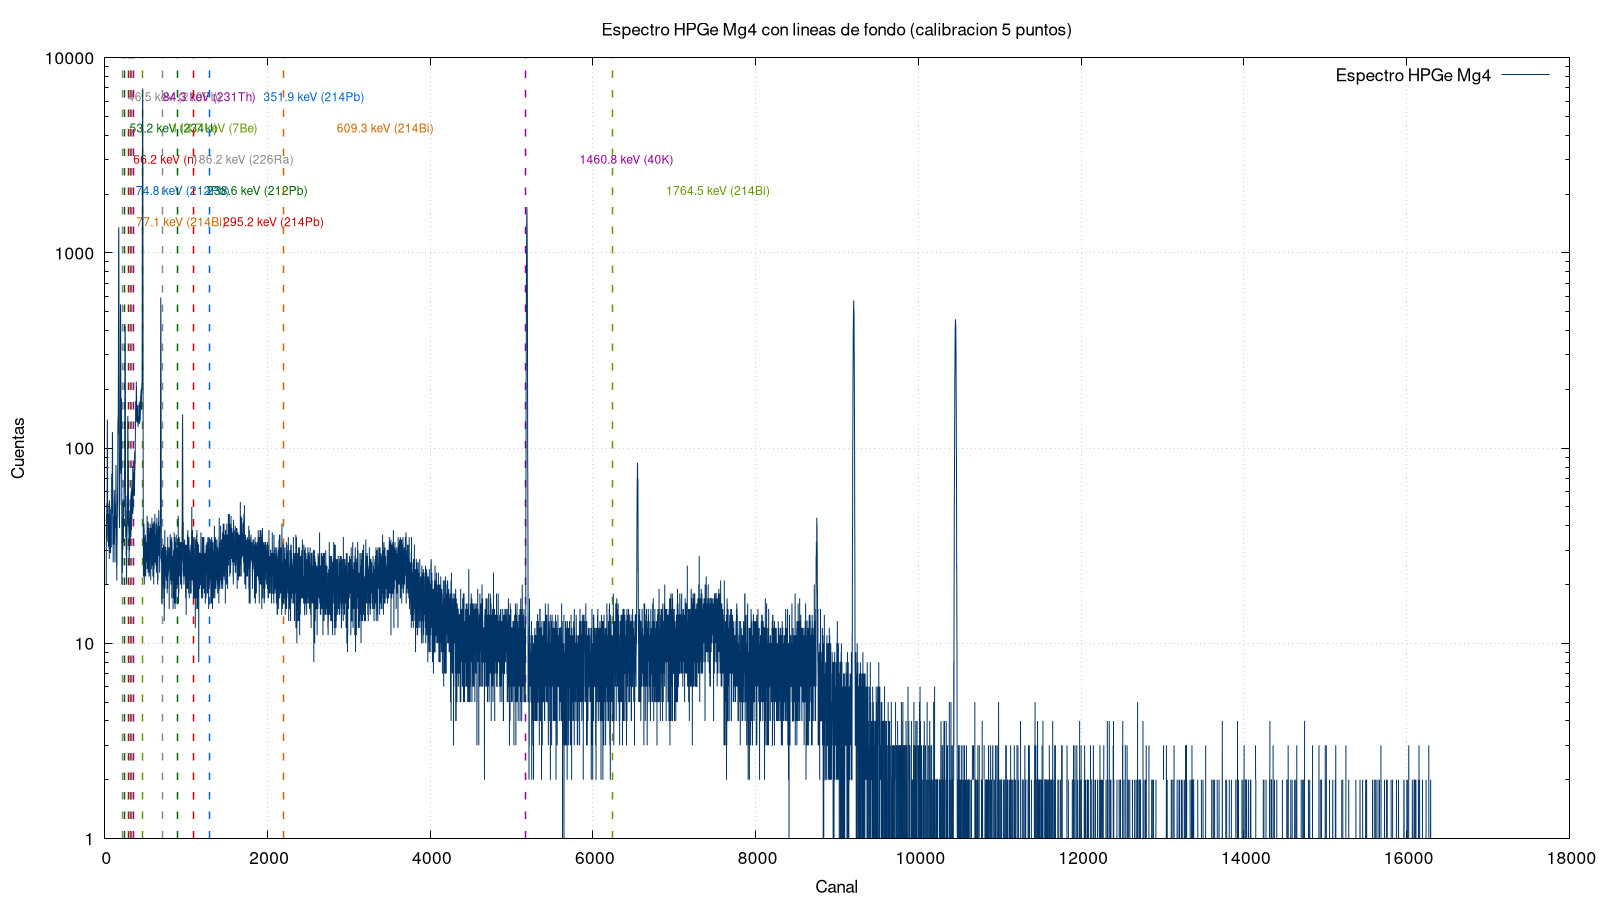
\includegraphics[width=0.95\textwidth]{plots/cal_hpge_full.png}
\caption{Espectro HPGe completo de Mg4 (escala logar\'{\i}tmica en cuentas).
Las l\'ineas verticales discontinuas marcan las posiciones predichas para
las 14 l\'ineas del fondo seg\'un la calibraci\'on multipunto
$E = -17.36 + 0.28568\cdot\text{canal}$.
Los picos de $^{40}$K (1460.8~keV, canal 5189) y $^{208}$Tl
(2614.5~keV, canal 9205) son claramente visibles;
el $^{214}$Bi a 1764.52~keV (canal 6237, cerca del l\'imite de detecci\'on)
no se distingue del ruido.}
\end{figure}

\section*{Pico de $^{40}$K: datos y ajuste}
\begin{figure}[h!]
\centering
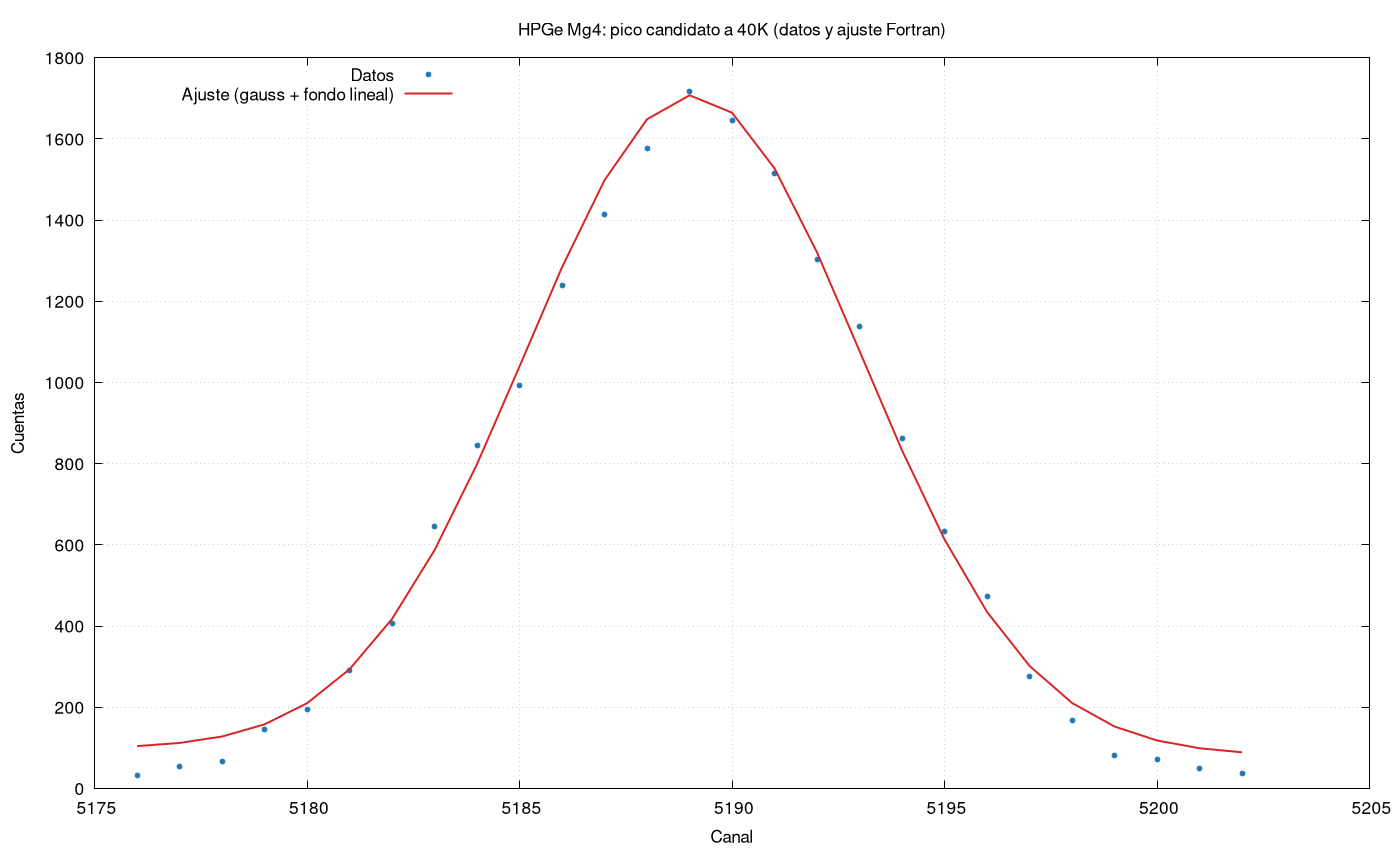
\includegraphics[width=0.95\textwidth]{plots/k40_hpge_fit.png}
\caption{Pico de $^{40}$K en el espectro HPGe de Mg4: datos experimentales
(puntos azules) y ajuste Fortran gaussiana+fondo lineal (l\'{\i}nea roja).}
\end{figure}

\newpage
\section*{Verificaci\'on en energ\'{\i}a}
En la siguiente figura se muestra el espectro completo calibrado en
energ\'{\i}a (0--2000~keV) con la calibraci\'on
$E(\text{keV}) = -17.3573 + 0.285675\cdot\text{canal}$.
Las l\'{\i}neas verticales marcan las energ\'{\i}as de referencia del archivo
\texttt{fondo\_GeHP\_BEGe.dat}.

\begin{figure}[h!]
\centering
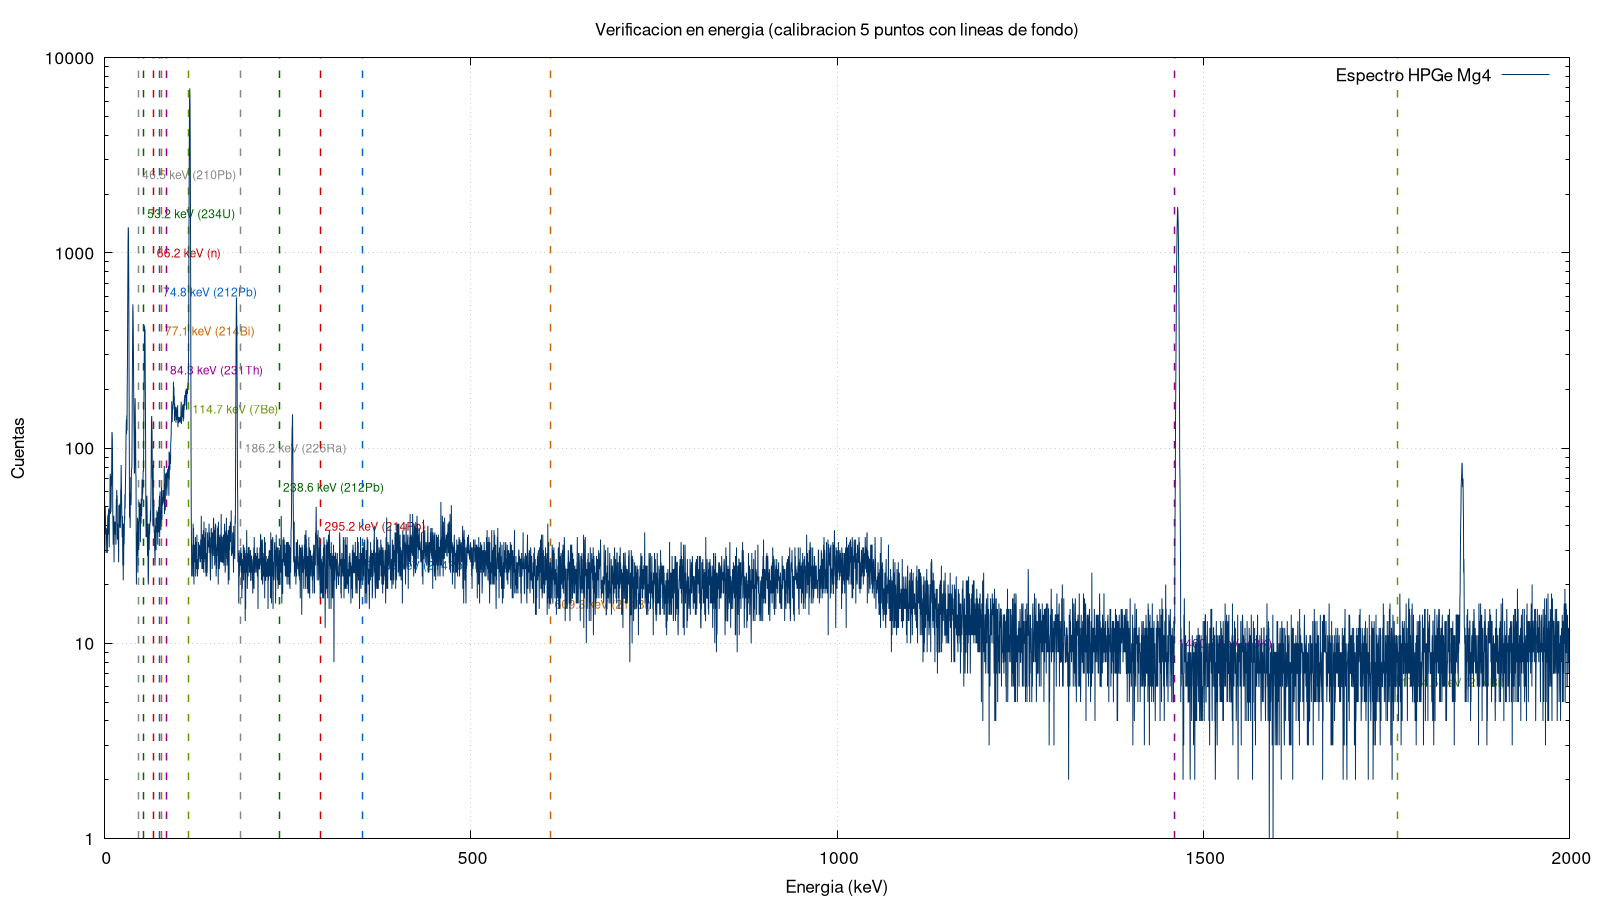
\includegraphics[width=0.95\textwidth]{plots/cal_hpge_verificacion.png}
\caption{Espectro HPGe de Mg4 calibrado en energ\'{\i}a con la calibraci\'on
multipunto de 5 anclas.
Las l\'{\i}neas verticales discontinuas marcan las energ\'{\i}as de referencia
de todas las l\'{\i}neas del fondo.
Se observa buena concordancia en la regi\'on de inter\'es alrededor de
1460~keV; las l\'ineas de baja energ\'{\i}a presentan desv\'{\i}os
sistem\'aticos por solapamiento espectral y no-linealidad residual.}
\end{figure}

\section*{Discusi\'on sobre la l\'{\i}nea de 1764.52~keV}
La l\'{\i}nea de 1764.52~keV ($^{214}$Bi) aparece en el fondo con una tasa de
96$\pm$16~cps$\cdot10^{-6}$, aproximadamente la mitad de la tasa de la
l\'{\i}nea de 609.31~keV (190$\pm$26~cps$\cdot10^{-6}$).
Sin embargo, en el espectro Mg4 no se distingue del ruido de fondo: el
m\'aximo local m\'as cercano al canal predicho (6237.4) se encuentra en el
canal 6251 con solo 18 cuentas (fondo $\sim$6--8).
Esto representa una contribuci\'on estad\'{\i}sticamente marginal,
consistente con la baja tasa esperada de esta l\'{\i}nea.

\section*{Conclusi\'on}
En el espectro HPGe de Mg4 se identifica un pico intenso en el canal
5189.086 cuyo ajuste gaussiano produce par\'ametros compatibles con un
fotopico bien definido de $^{40}$K.

La calibraci\'on en energ\'{\i}a se realiz\'o mediante regresi\'on lineal
de 5 anclas identificadas visualmente en el espectro:
$E(\text{keV}) = -17.3573 + 0.285675\cdot\text{canal}$
($R^2 = 0.999985$).
La l\'{\i}nea de $^{214}$Bi a 1764.52~keV no es detectable en Mg4
(canal predicho 6237.4, solo 18~cuentas contra fondo $\sim$6--8).

La verificaci\'on con las 14 l\'ineas de fondo muestra buena concordancia
general, con residuos $|\Delta E| < 4.4$~keV para las l\'ineas de
$E > 100$~keV que no presentan solapamiento. Se identificaron 6 l\'ineas con
discrepancias $>6$~keV, atribuibles a:
\begin{itemize}
  \item Solapamiento de m\'ultiples l\'ineas de fondo a baja energ\'{\i}a
    ($<100$~keV) que no pueden resolverse individualmente en este espectro
    (46.5, 74.8, 84.3~keV).
  \item Una peque\~na no-linealidad residual del sistema de adquisici\'on
    alrededor de 200--350~keV (186.2, 295.2, 351.9~keV).
\end{itemize}
Estas limitaciones son inherentes a una calibraci\'on lineal con l\'ineas de
fondo de baja estad\'{\i}stica en un espectro de activaci\'on neutr\'onica.

\end{document}
